\section{M-step}

The article miss at providing a full understanding on how Radial basis functions are used to compute exactly the M-step. In order to implement safely, it is of interest to write down all the analytic computations. So let's start from the beginning:\\

At iteration $k$, in the M-step, we assume that the joint states $(x_t, x_{t+1})$ and the joint state and output $(x_t, y_t)$ follow the laws:
\begin{align*}
  \left[ \begin{array}{c} x_{t}\\ x_{t+1}\\ \end{array} \right] &\sim
    \mathcal{N}\left(
      \left[ \begin{array}{c} \hat{x}_{t|T}\\ \hat{x}_{t+1|T}\\ \end{array} \right],
      \left[ \begin{array}{cc} \hat{P}_{t|T} & \hat{P}_{t,t+1|T}\\ \hat{P}_{t,t+1|T} & \hat{P}_{t+1|T}\\ \end{array} \right]
    \right),
    t=1 \ldots T-1\\
  \left[ \begin{array}{c} x_{t}\\ y_{t}\\ \end{array} \right] &\sim
    \mathcal{N}\left(
      \left[ \begin{array}{c} \hat{x}_{t|T}\\  f(\hat{x}_{t|T}, u_t)\\ \end{array} \right],
      \left[ \begin{array}{cc} \hat{P}_{t|T} & TODO \\ TODO & TODO\\ \end{array} \right]
    \right),
    t=1 \ldots T\\
\end{align*}
where the quantities $ \hat{x}_{t|T}, \hat{P}_{t|T}, \hat{P}_{t,t+1|T}$ were computed in the E-step.
We adopt the following notations :
\begin{align*}
  \mathcal{N}_{x_t} &= p(x_t)\\
  \mathcal{N}_{(x_t,x_{t+1})} &= p(x_t, x_{t+1})\\
\end{align*}

Now we want to compute the updated parameter $\theta^{(k)} = (\theta_f^{(k)}, \theta_g^{(k)})$ (and $Q$ and $R$.)\\ 

The updated parameter $\theta^{(k)}$ is the maximizer of the expected complete likelihood :
\begin{align*}
  \theta^{(k)} &= \underset{\theta}{\text{argmax }}L(\theta) = \underset{\theta}{\text{argmax }}l(\theta)\\
\end{align*}
where $l(\theta)$ is the expected log likelihood.
First we need to express $l(\theta)$ using the graph factorization.
Our graphical model is the following :
\begin{figure}[H]
	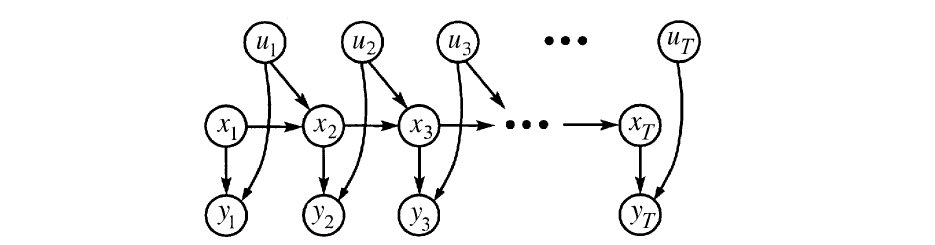
\includegraphics[width=14cm]{screenshot_graphical_model.PNG}
	\captionof{figure}{Graphical model of our system.}
\end{figure}
Firstly, the inputs $u_t$ are not modeled as random variable, so we won't take them into account in the factorization.
%\notes{If $u_t$ were random variables, we wouldn't have a tree anymore and the inference that we did in the E-Step would be complicated.}
Thus, the factorization over the graph yields :
\begin{align*}
p_{\theta}(x_1, \ldots x_T, y_1, \ldots , y_T) &= p_{\theta}(x_1) \prod_{t=1}^{T-1}{p_{\theta}(x_{t+1}|x_t)} \prod_{t=1}^{T}{p_{\theta}(y_t|x_t)}\\
\end{align*}
Thus, the likelihood of the observed the sequence $\overline{y} = (\overline{y}_t)_{t=1 \ldots T}$ is :
\begin{align*}
  p_{\theta}(x_1, \ldots x_T, \overline{y}_1, \ldots , \overline{y}_T) &= p_{\theta}(x_1) \prod_{t=1}^{T-1}{p_{\theta}(x_{t+1}| x_t)} \prod_{t=1}^{T}{p_{\theta}(\overline{y}_t, x_t)}\\
\end{align*}
Taking the $log$ and expectation of this likelihood over $x$ (whose unconditionnal law is known by assumption) gives us the expected log-likelihood:
\begin{align*}
  l(\theta) & =
    \mathbb{E}_x(\log(p_{\theta}(x_1))) +
    \sum_{t=1}^{T-1}{\mathbb{E}_x \left( \log(p_{\theta}(x_{t+1}|x_t)) \right)} +
    \sum_{t=1}^{T}{\mathbb{E}_x\left( \log(p_{\theta}(\overline{y}_t|x_t)) \right)}\nonumber \\
\end{align*}
These terms can be expressed in term our the $\hat{x}$ and $\hat{P}$ quantitites:
\begin{align*}
  \mathbb{E}_x(\log(p_{\theta}(x_1))) &= -\frac{1}{2}\int_x{\mathcal{N}_{x_1}(x) (x - \hat{x}_{1|1})^T \hat{P}_{1|1}^{-1} (x - \hat{x}_{1|1}) dx}\ (constant \  term)\\
  \mathbb{E}_x \left( \log(p_{\theta}(x_{t+1}|x_t)) \right) &= -\frac{1}{2}\int_{x,x'}{\mathcal{N}_{(x_t,x_{t+1})}(x, x') ((x' - f(x,u_t))^T Q^{-1} (x' - f(x,u_t)) dxdx'}\\
  \mathbb{E}_x\left( \log(p_{\theta}(\overline{y}_t|x_t)) \right) &= -\frac{1}{2}\int_x{\mathcal{N}_{x_t}(x) (\overline{y}_t - g(x, u_t))^T R^{-1} (\overline{y}_t - g(x, u_t)) dx}\\
\end{align*}
and the functions $f$ and $g$ can be expressed in terms of $\theta_f$ and $\theta_g$.\\

\textbf{We see that the expected log-likelihood is separable on $(\theta_f,Q)$, $(\theta_g,R)$ and that the terms $\mathbb{E}_x\left( \log(p_{\theta}(\overline{y}_t|x_t)) \right)$ and $\mathbb{E}_x(\log(p_{\theta}(x_{t+1}|x_t)))$ have the same form}.\\

In section 6.2.3 of the article, the authors explain how to deal with the maxization of terms of that form and give us a close form formula.
Firstly, to get rid of the multiplying constants $-\frac{1}{2}$, we multiply the expected log likelihood by $-2$ such that our maximization problem becomes a minimization problem :
\begin{align*}
  \theta^{(k)} &= \underset{\theta}{\text{argmin }}l(\theta)\\
\end{align*}
Introducing the author notations :
\begin{align*}
  \Phi_f(x, u) &= [\rho_1(x), \ldots , \rho_I(x), x^T, u^T, 1]^T\\
  \Phi_g(x, u) &= [\rho'_1(x), \ldots , \rho'_J(x), x^T, u^T, 1]^T\\
  \left< F(.) \right>_{x_t} &= \int_x{\mathcal{N}_{x_t}(x) F(x) dx} = \mathbb{E}_{x_t} \left( F(x) \right)\\
  \left< F(.) \right>_{x_t,x_{t+1}} &= \int_{x, x'}{\mathcal{N}_{(x_t, x_{t+1})}(x, x') F(x,x') dx}dx' = \mathbb{E}_{(x_t, x_{t+1})} \left( F(x, x') \right)\\
\end{align*} % NOTA : on ne devrait pas avoir les mêmes x et u pour f et g
such that:
\begin{align*}
  f(x,u_t) = \theta_f \Phi_f(x, u)\\
  g(x,u_t) = \theta_g \Phi_g(x, u)\\
\end{align*}
the expected log-likelihood minimization equation becomes:
\begin{align*}
  \left( \theta_f^{(k)},Q^{(k)} \right) &=
    \underset{\theta_f,Q}{\text{argmin }}{\left(
      \sum_{t=1}^{T-1}{\left< (x, x') \mapsto (x' - \theta_f\Phi_f(x,u_t)^T Q^{-1}(x' - \theta_f\Phi_f(x,u_t)) \right>_{x_t,x_{t+1}}+\log(|Q|)}
    \right)}\\
  \left( \theta_g^{(k)}, R^{(k)} \right) &=
    \underset{\theta_g,R}{\text{argmin }}{\left(
      \sum_{t=1}^{T}{\left< x \mapsto (\overline{y}_{t} - \theta_g \Phi_g(x, u_t))^T R^{-1} (\overline{y}_{t} - \theta_g \Phi_g(x, u_t)) \right>_{x_t}+\log(|R|)
    }\right)}\\
\end{align*}
and we are able to obtain the optimal parameters in close form:
\begin{align*}
  \theta_f^{(k)} &=
    \left(
      \sum_{t=1}^{T-1}{\left< (x,x') \mapsto x' \Phi_f(x,u_t)^T \right>_{x_t,x_{t+1}}}
    \right)
    \left(
      \sum_{t=1}^{T-1}{\left< x \mapsto \Phi_f(x, u_t)\Phi_f(x,u_t)^T \right>_{x_t}}
    \right)^{-1}
  \\
  \theta_g^{(k)} &=
    \left(
      \sum_{t=1}^{T}{\left< x \mapsto \overline{y}_{t}\Phi_g(x,u_t)^T \right>_{x_t}}
    \right)
    \left(
      \sum_{t=1}^{T}{\left< x \mapsto \Phi_g(x,u_t)\Phi_g(x,u_t)^T \right>_{x_t}}
    \right)^{-1}
    \\
\end{align*}
The interest of the RBF functions is that the expectations $\left< \ldots \right>_{x_t} = \mathbb{E}_{x_t} ( \ldots )$ and  $\left< \ldots \right>_{x_t,x_{t+1}} = \mathbb{E}_{(x_t, x_{t+1})}( \ldots )$ can be computed analatically and efficiently.
Otherwise, as soon as the state space dimension is big (for example $\geq 5$), these expectations must be estimmated, which is very expensive.

To compute $\theta_f^{(k)}$, we need to compute the expectations:
\begin{align*}
  \left< (x,x') \mapsto x' \Phi_f(x,u_t)^T \right>_{x_t,x_{t+1}} &=
    \left< (x,x') \mapsto [x'\rho_1(x), \ldots , x'\rho_I(x), x'x^T, x'u^T, x']\right>_{x_t,x_{t+1}}
  \\
  \left< x \mapsto \Phi_f(x, u_t)\Phi_f(x,u_t)^T \right>_{x_t} &=
    \left< x \mapsto \left[
      \begin{array}{cccc}
        (\rho_i(x)\rho_j(x))_{i,j} & x^T \rho_i(x) & u^T \rho_i(x) & \rho_i(x) \\
        \rho_j(x)x^T & x^T \rho_i(x) & u^T \rho_i(x) & TODO... \\
      \end{array}
    \right] \right>_{x_t}
  \\
\end{align*}
So we need to compute the elementary expectations:
\begin{align*}
  &\left< (x,x') \mapsto x'\rho_i(x) \right>_{x_t,x_{t+1}}\\
  &\left< (x,x') \mapsto x'x^T \right>_{x_t,x_{t+1}}\\
  &\left< (x,x') \mapsto x' \right>_{x_t,x_{t+1}}\\
  &\left< x \mapsto \rho_i(x)\rho_j(x) \right>_{x_t}\\
  &\left< x \mapsto x^T \rho_i(x) \right>_{x_t}\\
  &\left< x \mapsto \rho_i(x) \right>_{x_t}\\
  &\left< x \mapsto xx^T \right>_{x_t}\\
\end{align*}
We begin with the simple ones :
\begin{align*}
  \left< (x,x') \mapsto x'\right>_{x_t,x_{t+1}} &= \hat{x}_{t+1|T}\\
  \left< (x,x') \mapsto x'x^T\right>_{x_t,x_{t+1}} &= \hat{x}_{t+1|T}\hat{x}_{t|T}^T + \hat{P}_{t,t+1|T}\\
  \left< x \mapsto xx^T\right>_{x_t} &= \hat{x}_{t|T}\hat{x}_{t|T}^T + P_{t|T}\\
  \left< x \mapsto x\right>_{x_t} &= \hat{x}_{t|T}\\
\end{align*}
The expectations that involve RBF functions are more complicated to compute so we simply rewrite the formulas provided by the authors:
\begin{align*}
  \left<(x,x') \mapsto x'\rho_i(x)\right>_{x_t,x_{t+1}} &= TODO\\
  \left<x \mapsto \rho_i(x)\rho_j(x)\right>_{x_t} &= \\
  \left<x \mapsto x^T \rho_i(x)\right>_{x_t}\\
  \left<x \mapsto \rho_i(x)\right>_{x_t}\\
\end{align*}
